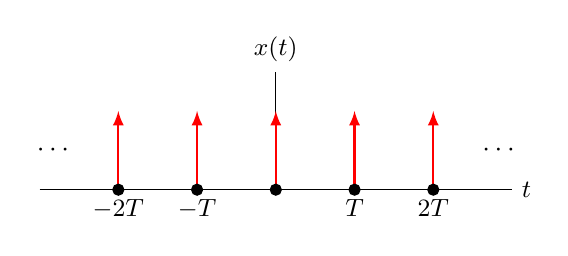
\begin{tikzpicture}
	\def\w{{-2, -1, 0, 1, 2}}
	\def\akmag{{1, 1, 1, 1, 1}}


	\begin{scope}	
		\draw (-3, 0) -- (3,0) node[anchor=west] {\small $t$};
		\draw (0, 0) -- (0,1.5) node[anchor=south] {\small $x(t)$};		
		\foreach \k/\l in {-2/{-2T}, -1/{-T}, 0/{}, 1/{T}, 2/{2T},}
		{
			\node at (\k, 0) [anchor=north] {\small $\l$};
		}
		%\node at (0,5) [anchor=south] {\small $Ta_k$};
		
		\foreach \k in {0,1, ..., 4}
		{
			\pgfmathparse{\w[\k]}
			\edef\wk{\pgfmathresult}
			\pgfmathparse{\akmag[\k]}
			\edef\akmagk{\pgfmathresult}	
			\draw[thick, red, -latex] (\wk, 0) -- ++(0,\akmagk);% node [anchor=south] {\small $\akmagk$};
			\ifthenelse{\lengthtest{0 pt = \akmagk pt}}{\draw[fill=black]  (\wk,0) circle (2pt);}{}
		}
			\node at (2.5, 0.5) [anchor=west] {$\cdots$};		
			\node at (-2.5, 0.5) [anchor=east] {$\cdots$};					
	\end{scope}
	\end{tikzpicture} 